\documentclass[12pt]{report}
\usepackage[utf8]{inputenc}
\renewcommand\thesection{\arabic{section}}
\usepackage[parfill]{parskip}
\usepackage{subcaption}
\usepackage{graphicx}
\usepackage[left=0.75in,right=0.75in,top=0.75in,bottom=0.75in]{geometry}
\usepackage{multirow}
\usepackage{hhline}
\usepackage{nth}
\usepackage{bm}
\usepackage{siunitx}
\usepackage{subcaption}
\usepackage[doublespacing]{setspace}
\usepackage{lineno} \linenumbers

\usepackage{xspace}
\newcommand{\GitHub}{\texttt{GitHub}\xspace}
\newcommand{\R}{\texttt{R}\xspace}
\newcommand{\natdb}{\texttt{NATDB}\xspace}

\usepackage{textcomp}
\usepackage{pifont}
\usepackage{minted}
\usepackage{hologo}

%%%%%%%%%%%%%%%%%%%%%%%%%%%%%%%%%%%
%Bibliography%%%%%%%%%%%%%%%%%%%%%%
%%%%%%%%%%%%%%%%%%%%%%%%%%%%%%%%%%%
\usepackage[citestyle=authoryear,bibstyle=authoryear,sorting=nyt,maxcitenames=2,maxbibnames=10,minbibnames=6,doi=false,url=false,isbn=false,firstinits=true,uniquename=false,uniquelist=false]{biblatex}
%Italicise et al.
\renewbibmacro*{name:andothers}{
% Based on name:andothers from biblatex.def
\ifboolexpr{ test{\ifnumequal{\value{listcount}}{\value{liststop}}} and test \ifmorenames } {\ifnumgreater{\value{liststop}}{1} {\finalandcomma}
{}%
\andothersdelim\bibstring[\emph]{andothers}} {}}
%Make 'and' an ampersand
\renewcommand*{\finalnamedelim}{%
\ifnumgreater{\value{liststop}}{2}{\finalandcomma}{}%
\addspace\&\space}
%Remove 'in:'
\renewbibmacro{in:}{}
%Remove pp. on pages numbers
\DeclareFieldFormat[article]{pages}{#1}%
%Remove unwanted entries
\AtEveryBibitem{%
  \clearfield{day}%
  \clearfield{month}%
  \clearfield{endday}%
  \clearfield{endmonth}%
  \clearfield{url}%
  \clearfield{URL}%
  \clearfield{eprint}%
}
%Remove spaces between initials
%Remove double quotes around titles
\DeclareFieldFormat*{citetitle}{#1}
\DeclareFieldFormat*{title}{#1}
\addbibresource{Library.bib}
%%%%%%%%%%%%%%%%%%%%%%%%%%%%%%%%%%%

\begin{document}
\section*{Title page}
\textbf{Article title}: \natdb : An \R package that downloads species
trait data, but is Not A Trait DataBase

\textbf{Running head}: \natdb: Not A Trait DataBase

\textbf{Authors:} William D.\ Pearse$^{1,2,*}$, Maxwell J.\
Farrell$^3$, Konrad Hafen$^4$, Mallory Hagadorn$^1$, Spencer B.\
Hudson$^1$, Sylvia Kinosian$^1$, Ryan McCleary$^1$, Alexandre
Rego$^1$, \& Katie Welgarz$^1$

$^1$Department of Biology, Utah State University, 5305 Old Main Hill,
Logan UT, 84322, USA

$^2$Ecology Center, Utah State University, 5305 Old Main Hill, Logan
UT, 84322, USA

$^3$ Biology Department, McGill University, 1205 Docteur Penfield,
Montreal, QC H3A 1B1, Canada

$^4$Department of Watershed Science, Utah State University, 5305 Old
Main Hill, Logan UT, 84322, USA

$^*$To whom correspondence should be addressed:
\url{will.pearse@usu.edu}

\textbf{Keywords}: traits, database, \R, open science, taxonomy

\textbf{Word-count}: XXX

\clearpage
\section{Abstract}
\begin{enumerate}
\item Ecologists and evolutionary biologists often wish to make use of
  species trait data, either as ancillary data, such as in community
  ecology, or as the primary focus of a study, such as
  macro-evolutionary modelling.
\item Such biologists are often hampered by the difficulties of
  collecting sufficient trait data from published sources.
\item We present \natdb, an \R package that automatically downloads
  species trait data from existing sources.
\item NATDB collates trait data from over 100 publications across
  $\mathtt{\sim}120,000$ species, and at the time of writing downloads
  over 3.5 million individual trait measurements.
\item NATDB is \emph{Not A Trait DataBase}: it circumvents issues over
  the intellectual ownership of data by distributing no data, and
  merely giving users automated tools to create their own database
  from data that scientists have already agreed to share. We hope to
  establish a community around this package that will add additional
  data sources and cleaning routines.
\item \natdb can be installed by typing
  \texttt{library(devtools);install\_github("willpearse/natdb")} at an
  \R console. We will submit the package to CRAN once it is accepted
  at a journal.
\end{enumerate}

\clearpage
\section{Introduction}
Ecologists and evolutionary biologists have long recognised the
importance of (functional) traits in their work \autocite{Diaz2001}.
Biodiversity is a multi-faceted concept \autocite{Purvis2000}, but it
is intuitively obvious that if we are to understand patterns in
biodiversity and the processes that govern it, we must have
quantitative data on the properties of species themselves. Large
datasets of plants \autocite{Kattge2011}, mammals
\autocite{Jones2009}, and birds \autocite{Wilman2014} have opened the
door to analyses of the evolution \autocite{Harmon2010a,Pennell2015}
and global distribution \autocite{Kattge2011,Gross2017} of trait
diversity.  Species' traits help us better predict how species will
respond to land use \autocite{Mayfield2010a} and climate change
\autocite{Estrada2016}, allowing us to generalise and compare across
species to find general biodiversity patterns.

Yet, despite its importance, it is often difficult to find data on
species' functional traits. We suggest there are three main reasons
for this: (1) it is difficult to obtain trait data, (2) it is
difficult to collate trait data, and (3) trait data are not always
published. (1) Often the most functionally important species traits
are the most difficult to measure
\autocite{Cornelissen2003,Violle2007}, and even when measuring a trait
is simple, finding a suitable specimen is often not. Usefully
measuring and defining species' traits requires specialist knowledge
and expertise, and is difficult to do properly. If a solution exists
to this problem, it is likely a re-allocation of funding towards
training biologists capable of measuring species' traits. While
advances in machine learning improve the prospects of automated trait
collection \autocite[\emph{e.g.},][]{Pearse2016}, methods for easing
data collection will most likely vary across species and traits: there
will be no single silver-bullet solution.

The last two of the problems above, however, may be possible to tackle
across all species and traits simultaneously. (2) Creating and
maintaining large databases is complex: the nomenclatures for species
and traits are not universal \autocite{Kattge2011,Hudson2017}, and
resolving discrepancies across datasets requires detailed knowledge of
species and their traits. A potential solution, however, is to develop
a framework within which it is possible for this specialist-driven,
intensive discrepancy resolution to be parallelised across many
scientists. Focusing on the development not of a database \emph{per
  se}, but rather on the tools that enable the creation of databases,
may allow this. The modern data scientist makes frequent use of tools
such as \GitHub \autocite[reviewed in][]{Ram2013}, which are designed
to ease decentralised effort on common tasks such as nomenclature
resolution. (3) Unlike other other kinds of data such as DNA sequences
\autocite{Benson2013}, the publication of species trait data has been
controversial \autocite[\emph{e.g.},][]{Moles2013,Poisot2013}. The
most compelling argument against the publication of data is a concern
that a database creator, with a few minutes' work, could grab data
that took decades to collect, and receive all the citation credit for
that data as released in what we call a ``\emph{pseudo-new}''
dataset. This objection would be resolved if scientists didn't use (or
create) such pseudo-new datasets, and instead cited the sources of the
original data that they make use of.

We present here \natdb, an \R package that collates over 3.5 million
trait records for $\mathtt{\sim}120,000$ species, making existing
species trait data more widely available for use by ecologists and
evolutionary biologists. We argue that \natdb is a prototype for a new
way of making data more accessible that avoids concerns about data
ownership and pseudo-new datasets: \natdb is \emph{Not A Trait
  DataBase}. \natdb is a software package that simplifies the process
of collating data the user already has access to, and so obviates any
concerns over attribution in pseudo-new dataset because it simply
retrieves data whose collectors have already publicly released. \natdb
contains no data, and so users must cite the sources of data when
using the package. This model both liberates the vast trait-based
knowledge that already exists in the literature, and protects the
intellectual contributions of those who collected the data in the
first place.

\clearpage
\section{Usage}
\natdb consists of a series of internal functions, each of which
downloads a single dataset from a published source. Typically, a user
will download a set of data and then subset that down to only the
species or traits that they require. Note that, by default, \natdb
waits ten seconds between downloading datasets to minimise impact on
journals' servers. For example, the following would download all the
data in \natdb, and then subset that down to only two kinds of traits
for two species:

\begin{minted}{splus}
  library(natdb)
  data <- natdb(taxon)
  species <- c("Quercus_robur", "Pinus_sylvestris")
  traits <- c("specific_leaf_area", "height")
  subset.data <- data[species, traits]
\end{minted}

\natdb can cache whatever it downloads during an \R session. So, for
example, if the user were to realise that they wanted data on an
additional species or trait after executing the code above, they could
run the entire script again and \natdb would not download any more
data. To use this option, a user must specify a directory when
invoking \natdb so that they can save their searches between
sessions. The following code, for example, would cache results between
sessions, and would add additional data to that cache as new versions
of \natdb were released. This is the recommended way to use \natdb, as
it saves the user time and reduces server load.

\begin{minted}{splus}
  data <- natdb(cache="~/.natdb_cache/")
  subset.data <- data[c("Phocoena_phocoena","Tursiops_truncatus"),]
\end{minted}

\natdb has a single class for dealing with trait data, called
(unimaginatively) \texttt{natdb}. This class has \texttt{head},
\texttt{print}, \texttt{summary}, and \texttt{as.data.frame} methods
to make it easier for the user to work with their data. Internally,
\natdb distinguishes between, and convert all data into,
\texttt{numeric} and \texttt{character} types, and \emph{melts}
\autocite[\emph{sensu}][]{Wickham2007} all data within these
types. This makes it easy to add new data to an existing \natdb
object, and keeps the memory requirements manageable. If \natdb were
to store data in a \texttt{data.frame}-like format, it would require
$\mathtt{\sim}14,400,000,000$ cells ($\mathtt{\sim}120,000$ species,
$\mathtt{\sim}1,200$ traits) to store all its data, $\mathtt{\sim}2\%$
of which would be empty. Users are encouraged to explore options for
summarising the data in \natdb, as the means and modes reported for
the \texttt{numeric} and \texttt{character} data, respectively, may
not be best-suited for their particular needs.

Ready access to meta-data is important in any database. The databases
\natdb can build are complex, in that the meta-data that different
source datasets provide can vary a great deal. We follow the general
approach of \emph{FigShare} (\url{https://figshare.com/}) and
\emph{DataDryad} (\url{http://datadryad.org/}) in not enforcing rigid
meta-data requirements, but placing the meta-data of each source
dataset within a comparable framework so as to allow users to
interrogate the meta-data in their own way. Thus while we do
standardise some aspects of the data (\emph{e.g.}, ensuring all
latitude and longitude measurements, where present, are termed
\texttt{latitude} and \texttt{longitude}), users must check whatever
subset of data they have to see what meta-data are available. For
example:

\begin{minted}{splus}
  simplified.data <- as.data.frame(subset.data)
  simplified.metadata <- metadata(subset.data)
  plot(simplified.data$specific_leaf_area ~ metadata$latitude)
\end{minted}

We make no guarantee that the taxonomy or units of the data within
\natdb are internally compatible: users are responsible for checking
the validity of the data they have collated. However, we have made
attempts to harmonise trait names within \natdb, and provided wrapper
scripts that use \texttt{taxize} and \texttt{convertr} to harmonise
taxonomy and units, respectively. For example:

\begin{minted}{splus}
  data <- natdb(taxon)[c("Quercus_robur", "Pinus_sylvestris"), ]
  # Basic cleaning (of trait, species, and unit names)
  clean.data <- clean.natdb(data)
  # Clean taxonomy using Global Names Resolver through taxize
  clean.data <- clean.natdb.names(clean.data)
  # Convert traits to a single unit of measurement
  clean.data <- clean.natdb.units(clean.data)
\end{minted}

Finally, it is important that those who generated the data \natdb
downloads are appropriately cited. It is simple to generate
\hologo{BibTeX} files to help with citations; for example:

\begin{minted}{splus}
  citations(clean.data)
\end{minted}

\clearpage
\section{Coverage and scope}
As table \ref{overview} shows, \natdb downloads data from over 100
published papers, and covers a reasonably wide range of taxonomic
groups (including, but not limited to, plants, birds, mammals,
amphibians, and reptiles). In terms of species- and trait-level
coverage, over 200 traits have data on over 1000 species (see figure
\ref{coverage}). We emphasise that more rigorous taxonomic cleaning
(and trait definition checking) may somewhat alter these figures (see
also below). Critically, \natdb has been designed, from the ground-up,
to be easy to extend. Adding a publication's data to the package
requires no knowledge other than the basic structure of data to be
added. Many of the functions that load data structure into \natdb are
fewer than ten lines of \R code, in part because we have contributed
code to the \R package \texttt{fulltext} \autocite{Chamberlain2015} to
automate the download of data from published papers. Since \natdb uses
reflective programming to determine what datasets are available for
download, all a user need do to add a dataset to \natdb is submit a
`pull request' on \GitHub with a function. This represents a major
advantage to \natdb: it is a living package that will, we hope, grow
as authors add their own publications to it. We provide detailed
instructions on how to contribute data sources to \natdb in the
package's vignette and on the package's \GitHub wiki.

The flexibility and scope of \natdb, however, means its output has not
been as carefully cleaned and checked as most published datasets
typically are. This is by design: \natdb is fundamentally different,
and we use the TRY dataset \autocite{Kattge2011} to illustrate
this. TRY is a carefully-collated dataset that required thousands of
person-hours to create, and to reflect this and ensure that the data
is used correctly, its authors require that many data contributors and
the two lead authors of the database are offered co-authorship on any
publication making use of TRY data. We consider this reasonable
request given the amount of effort involved in producing a database
like TRY, and the feedback and data-validation that these additional
co-authors provide to a finished manuscript. But \natdb is not a
database and does not follow this model: the data are provided `as-is'
and neither we, nor the original data publishers, require
co-authorship for use of the package.

\clearpage
\section{Future directions}
We actively encourage code contributions, and the package's online
vignette contains a detailed set of instructions on how to contribute
functions that download data from new sources. Our intention is to
make the process as simple as possible, and so encourage authors to
release the data underlying their analyses and integrate them into the
package. We hope that this will speed scientific development by making
data more widely available for analysis, and increase the rate at
which those who collect data can be acknowledged and cited for their
effort. This, in part, is the reason we have few formal checks on
meta-data and units within \natdb: the first hurdle we must overcome
is getting data `out there' in a useable format, and everything else
is a problem for the future. We hope that, using \natdb as a base,
others will develop cleaning and checking routines that can be applied
to the data the package downloads. Whether these will be incorporated
into \natdb itself, or released as separate companion package(s),
remains to be seen.

Without data there can ultimately be no science, and we hope \natdb
will make it easier to access data and to acknowledge those who
collected it. \natdb is an experiment, and its long-term success or
failure will depend on whether we can develop around it a community of
scientists willing to share their data through it.

\clearpage
\printbibliography

\clearpage
\section*{Figures}
\begin{figure}[h!]
  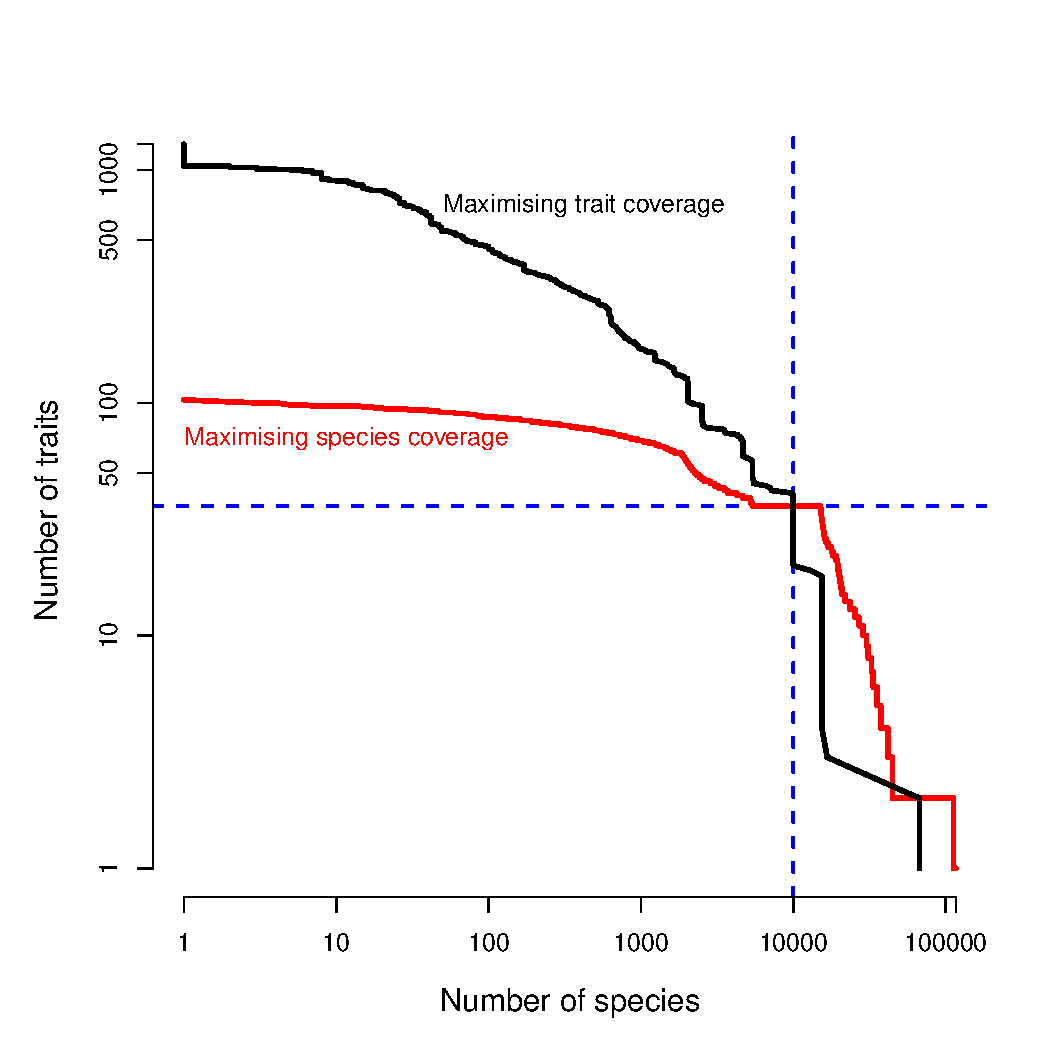
\includegraphics[width=.8\textwidth]{coverage.pdf}
  \caption{\doublespacing Data coverage within \natdb. Within \natdb,
    no species has data for every trait, and no trait has data for
    every species.  Thus while \natdb downloads over 3.5 million
    pieces of data, this number is not necessarily representative of
    the species- or trait-coverage can expect to work with. Since it
    is possible to select groups of species or traits within \natdb
    maximising the number of species or traits for which data are
    available, we plot coverage curves maximising species (in red) and
    traits (in black). The point of intersection between the two
    curves (at $10,000$ species and $36$ traits) is shown with blue
    dashed lines. This plot was produced using data that had been run
    through \natdb's \texttt{clean.natdb} function to harmonise trait
    and (to a limited extent) species names.}
  \label{coverage}
\end{figure}

\clearpage
\section*{Tables}
\begin{table}[h!]
  \begin{tabular}{lllll}
    Taxonomic group & \# Species & \# Traits & \% Complete & Citations \\ \hline
    Plants & & & \textcite{Wright2004}\\
    Mammals & & & \textcite{Jones2009,Wilman2014}\\
    Birds & & & \textcite{Wilman2014}\\
    ...TBC... \\ \hline
  \end{tabular}
  \caption{Overview of data available for download within
    \natdb. Overall, the package downloads XXX data points, covering
    XXX species and XXX separate functional traits. XXX\% of these
    trait values have some form of meta-data associated with them.}
  \label{overview}
\end{table}

\end{document}
%%% Local Variables:
%%% mode: latex
%%% TeX-master: t
%%% End:
